% @Author: AnthonyKenny98
% @Date:   2020-02-26 09:00:23
% @Last Modified by:   AnthonyKenny98
% @Last Modified time: 2020-04-09 13:40:11

% INTRO
To recap, the bottleneck function of a common motion planning algorithm, \gls{RRT}, was identified as edge collision detection. The functional hardware unit, HoneyBee, successfully accelerated this function by almost 5 times. The last two objectives of this thesis were:
    \begin{itemize}
    \item To define a RISC-V Extension Instruction Set for the purposes of accelerating motion planning.
    \item To verify the RISC-V Extension and the functional hardware unit in a complete RISC-V Processor.
    \end{itemize}

\section{Computer Architecture Background}
    % @Author: AnthonyKenny98
% @Date:   2020-03-01 19:39:42
% @Last Modified by:   AnthonyKenny98
% @Last Modified time: 2020-04-10 08:08:38

% Intro
Computer Architecture encompasses the design of the Instruction Set Architecture and Microarchitecture of a computer. The Instruction Set defines an abstract model of a computer, i.e. how it behaves. Microarchitecture is the implementation of this abstract model, i.e. desiging a CPU to execute the behavious specified in the instruction set.

% @Author: AnthonyKenny98
% @Date:   2020-04-09 10:47:05
% @Last Modified by:   AnthonyKenny98
% @Last Modified time: 2020-04-09 11:21:26
\begin{figure}[H]
\begin{centering}
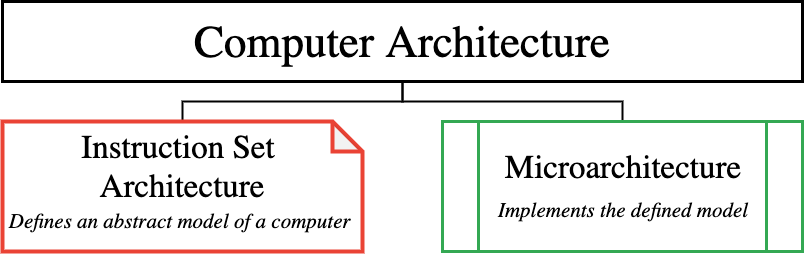
\includegraphics[width=0.7\linewidth]{chapters/chapter4/img/architecture.png}
\mycaption{Overview of the Field of Computer Architecture}{}
\end{centering}
\end{figure}

\subsection{Instruction Set Architecture}
    An \glsfirst{ISA} is an abstract model of a computer. On a broad level, it defines the data types, memory model, and registers of a computer, along with the instructions that it can execute. \\
    In more human terms, it can be thought as a ``contract'' between hardware and software developers. It is the promise made that the hardware will be able to execute all instructions defined in the \gls{ISA}, and the limitation that software must be compiled into that set of instructions.

    % @Author: AnthonyKenny98
% @Date:   2020-04-09 10:47:05
% @Last Modified by:   AnthonyKenny98
% @Last Modified time: 2020-04-11 01:21:24
\begin{figure}[H]
\begin{centering}
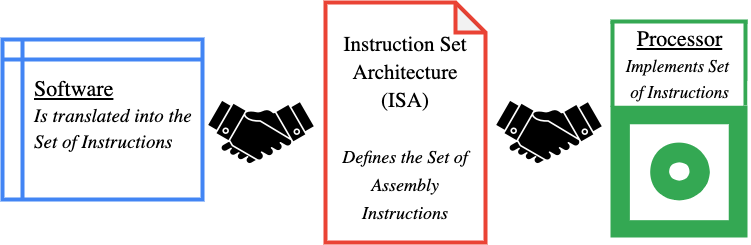
\includegraphics[width=\linewidth]{chapters/chapter4/img/contract.png}
\mycaption{The ISA is a Contract Between Software and Hardware Developers}{}
\end{centering}
\end{figure}

    The two most important things an \gls{ISA} defines are a computers \textbf{registers} and \textbf{instructions}. Instructions are the operations the computer can execute. Consider the \texttt{add} instruction: 
    \begin{center}
    \texttt{add rd, rs1, rs2}
    \end{center}

    This instruction computes \texttt{rs1} $+$ \texttt{rs2} and stores the result in \texttt{rd}.  (Where \texttt{rd}, \texttt{rs1}, and \texttt{rs2} are all \textbf{registers}).
    

\subsection{RISC Microarchitecture}
    
    \gls{RISC} is a broad category of \glspl{ISA}. Appendix \ref{section:philv_appendix_risc} gives a background on RISC principles. Figure \ref{fig:RISC-Datapath} shows the most simple layout of a 5-stage \gls{RISC} Datapath. In the \textbf{Instruction Fetch} stage, the processor gets the next instruction from memory for it to be decoded in the \textbf{Instruction Decode} stage. Here, the instruction is split into its constituent parts and has certain minor operations performed that are neccesary for the next stage. The \textbf{Execution} stage is where most computation occurs. This is where the \glsfirst{ALU} resides, and the result of this computation goes to the \textbf{Memory} stage. This is where values are stored into or loaded from the processor's memory, these values, or the values from the Execution stage, are saved to one of the processor's registers in the \textbf{Writeback} stage. 
    % @Author: AnthonyKenny98
% @Date:   2020-03-01 20:09:46
% @Last Modified by:   AnthonyKenny98
% @Last Modified time: 2020-04-03 13:32:58
\begin{figure}[H]
    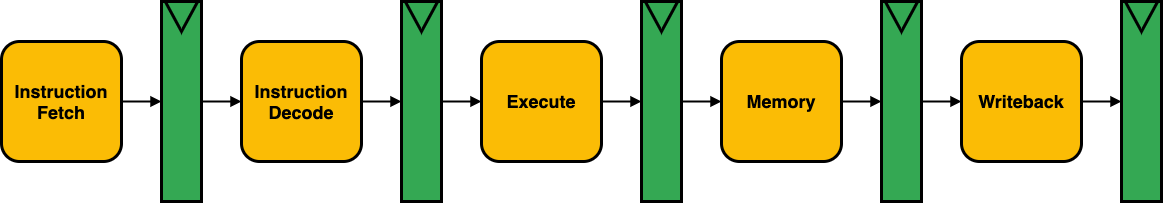
\includegraphics[draft=false,width=\linewidth]{chapters/chapter4/img/RISC-Datapath.png}
    \caption{5-Stage \gls{RISC} Datapath}
    \label{fig:RISC-Datapath}
\end{figure}


\newpage
\section{RISC-V Instruction Set}
    % @Author: AnthonyKenny98
% @Date:   2020-03-01 18:51:24
% @Last Modified by:   AnthonyKenny98
% @Last Modified time: 2020-03-01 19:39:08
\subsection{RV32I}

        The following is an excerpt from the RISC-V Specification, outlining the RV32I base integer instruction set \cite{Waterman2019}
        \begin{quote}{}
            \small{RV32I was designed to be sufficient to form a compiler target and to support modern operating system environments. The ISA was also designed to reduce the hardware required in a minimal implementation. RV32I contains 40 unique instructions, though a simple implementation might \dots [reduce] base instruction count to 38 total. RV32I can emulate almost any other ISA extension \dots \\
            Subsets of the base integer ISA might be useful for pedagogical purposes, but the base has been defined such that there should be little incentive to subset a real hardware implementation \dots}
        \end{quote}

        \subsubsection*{Registers}
        RV32I defines 32 unprivileged registers, each 32 bits wide. They are designated \texttt{x0-x31}, where \texttt{x0} is a hard-wired value of $0$, and registers \texttt{x1-x31} hole values that various instructions use. RISC-V uses the load-store method, meaning that all operations perform on two registers or a register and an immediate, rather than performing operations directly on memory addresses. In addition, the 33rd unprivileged register is the program counter \texttt{pc}. Table \ref{table:rv32i_reg} shows the register state for the RV32I Base Integer Instruction Set.
        % @Author: AnthonyKenny98
% @Date:   2020-03-01 18:36:35
% @Last Modified by:   AnthonyKenny98
% @Last Modified time: 2020-03-01 19:33:20
\begin{table}[H]
\begin{center}
\begin{tabular}{|p{.15\linewidth}|p{.15\linewidth}|p{.4\linewidth}|}
    \hline
    \textbf{Register}   & \textbf{ABI Name}  & \textbf{Description} \\
    \hline
    \texttt{x0}  & \texttt{zero} & Hard-wired zero \\
    \texttt{x1}& \texttt{ra}& Return address\\
    \texttt{x2}& \texttt{sp} & Stack pointer\\
    \texttt{x3}& \texttt{gp}&Global pointer\\
    \texttt{x4}& \texttt{tp}& Thread pointer\\
    \texttt{x5-7}& \texttt{t0-2}&Temporaries\\
    \texttt{x8}& \texttt{s0/fp}&Saved register/Frame pointer\\
    \texttt{x9}&\texttt{s1} &Saved register\\
    \texttt{x10-11}&\texttt{a0-1}&Function arguments/return values\\
    \texttt{x12-17}&\texttt{a2-7}&Function arguments\\
    \texttt{x18-27}&\texttt{s2-11}&Saved registers\\
    \texttt{x28-31}&\texttt{t3-6}&Temporaries\\
    \hline
    \texttt{pc} & \texttt{pc} & Program counter \\
    \hline
\end{tabular}
\caption{Register State for RV32I Base Instruction Set}
\label{table:rv32i_reg}
\end{center}
\end{table}

        \subsubsection{Instruction Formats}
        Table \ref{table:rv32i_instr_format} demonstrates the format of each different instruction type. 
        % @Author: AnthonyKenny98
% @Date:   2020-03-01 19:13:03
% @Last Modified by:   AnthonyKenny98
% @Last Modified time: 2020-03-01 19:32:00
\begin{table}[H]
\begin{center}
    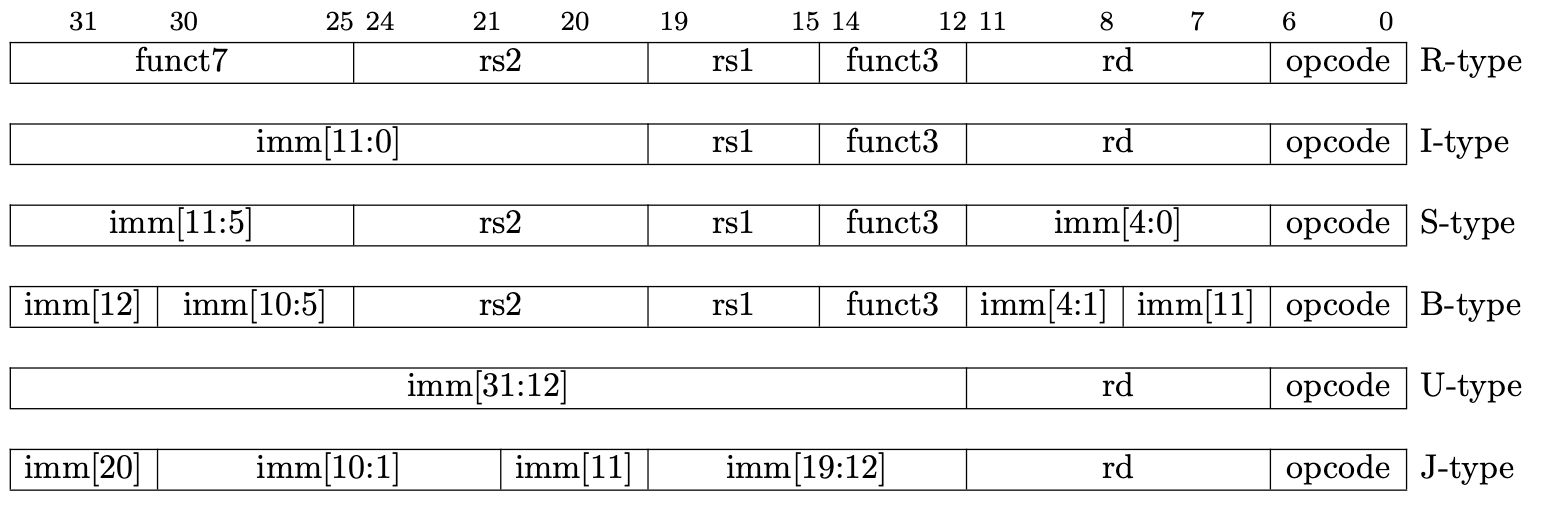
\includegraphics[draft=false,width=\linewidth]{chapters/chapter4/img/rv32i_instr_format.png}
    \caption{RV32I Base Instruction Formats}
    \label{table:rv32i_instr_format}
\end{center}
\end{table}



    \subsection{Motion Planning Extension}
        \todo[inline, caption={Motion Planning Extension}]{Full description of design of Non standard extension for motion planning. Should follow define, design, build, measure, analyse etc format.}

\newpage
\section{PhilosophyV}
    % @Author: AnthonyKenny98
% @Date:   2020-04-09 10:22:31
% @Last Modified by:   AnthonyKenny98
% @Last Modified time: 2020-04-10 08:08:13
\textit{Philosophy 4}, written in 1903 by Mr. Owen Wister of the Class of 1882 (founder of the Western literary genre), recounts the antics of two Harvard students and their last minute attempts to study (or avoid studying) for a Philosophy exam for which they are hopelessly unprepared. Similarly, this section details the process of building a RISC-V processor, by far the most intricate engineering challenge of this Thesis, and a task for which I was unsure of my preparedness. As such, this processor was named \textbf{PhilosophyV}; both in reference to the RISC-V ISA for which it was designed, and to the fact that the process of its implementation at times seemed very much like a sequel to Mr. Wister's novel. \\

The purpose of implementing a functional RISC-V processor was to verify that the design of the Xedgcol extension was viable. Initially, the hope was to find an existing open-source implementation, of which there are many, that I could build on. A significant period of time was spent trying to become familiar with the Rocket Core\cite{ChipsAlliance2020}, a large open-source RISC-V implementation. However, the project was so sophisticated that learning its infrastructure and the neccesary tool-chains became a massive project in itself. This was the case for many open-source projects. Those that lacked such sohpisticated code bases also lacked proper documentation and were not verified to be correct. As a result, it ended up being faster and simpler to implement a lightweight RISC-V processor from scratch. 

    \subsection{RV32I Implementation}
        % @Author: AnthonyKenny98
% @Date:   2020-04-09 20:56:24
% @Last Modified by:   AnthonyKenny98
% @Last Modified time: 2020-04-10 06:41:52
\begin{figure}[H]
\begin{center}
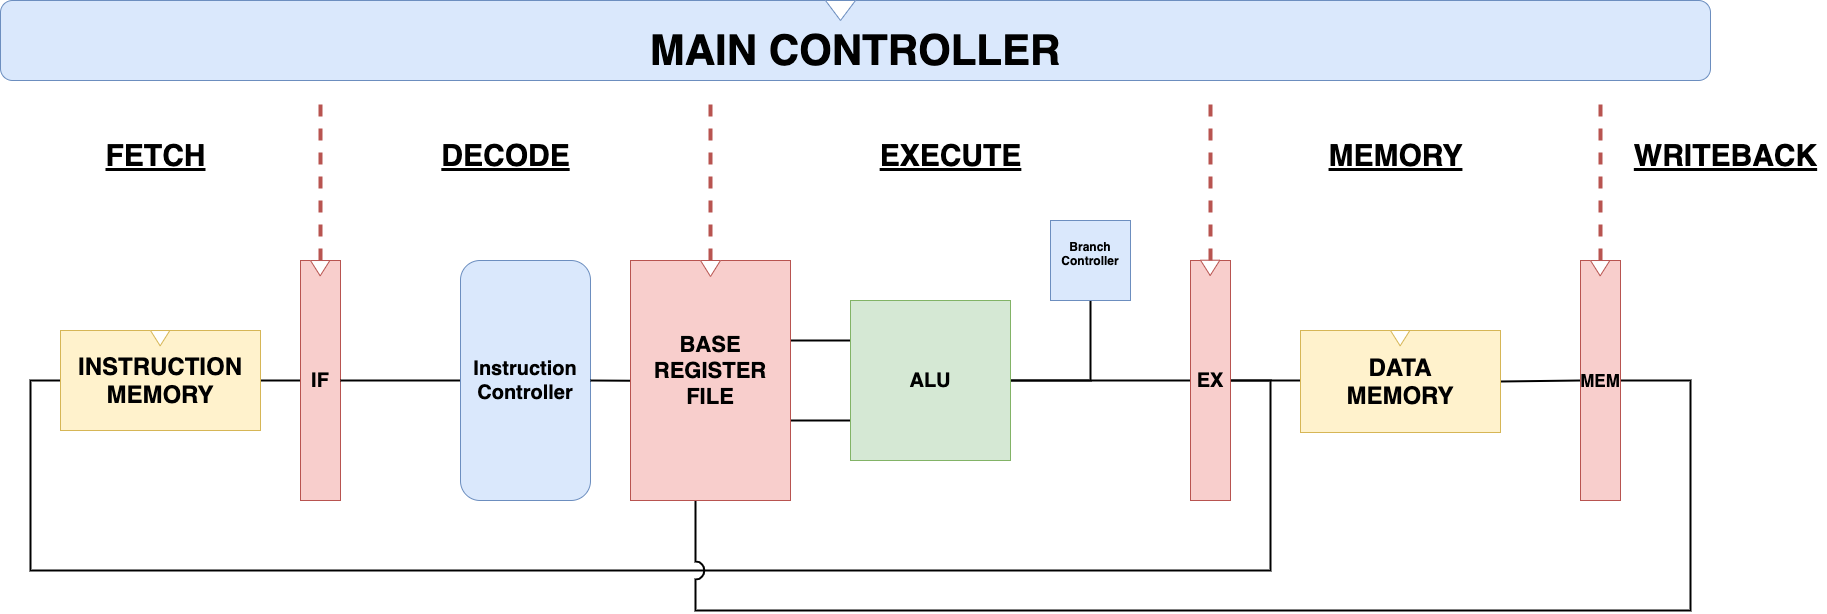
\includegraphics[width=\textwidth]{chapters/chapter4/img/philv_rv32i.png}
\mycaption{Simplified Schematic of the RV32I PhilosophyV Core}{}
\label{fig:philv_rv32i}
\end{center}
\end{figure}
        The first step was implementing a simple (a relative term) processor that implemented the RV32I Base ISA. Figure \ref{fig:philv_rv32i} shows a highly simplified schematic of the RV32I PhilosophyV Core. Appendix \ref{section:philv_appendix_rv32i_core} provides a detailed schematic.

        The design was that of a simple 5-stage non-pipelined processor with no branch-prediction or other optimizations. In other words, it's awful. Running the original \gls{RRT} program on this processor would take an inordinate amount of time (luckily, this was never tested). However, this is irrelevant. The improved performance of implementing the edge collision detection function in hardware has already been verified against an Intel processor that was designed by some of the leading minds in computer architecture. To restate, the purpose of implementing this processor was simply to prove the validity of the Xedgcol ISA extension.

        The processor was implemented in Verilog (an \gls{HDL}). Simulations were carried out in Vivado Design Suite. The processor's  correctness was verified at the module level and at the core level. Module testing was fulfilled by Verilog test benches that checked the functional correctness of each module (e.g. the ALU). The overall core was tested by running different complex assembly programs through the processor and comparing the states of its memory and register file at the end of the programs execution to their expected states.

    \subsection{RV32I\_Xedgcol Implementation}
        % @Author: AnthonyKenny98
% @Date:   2020-04-09 20:56:24
% @Last Modified by:   AnthonyKenny98
% @Last Modified time: 2020-04-10 06:41:49
\begin{figure}[H]
\begin{center}
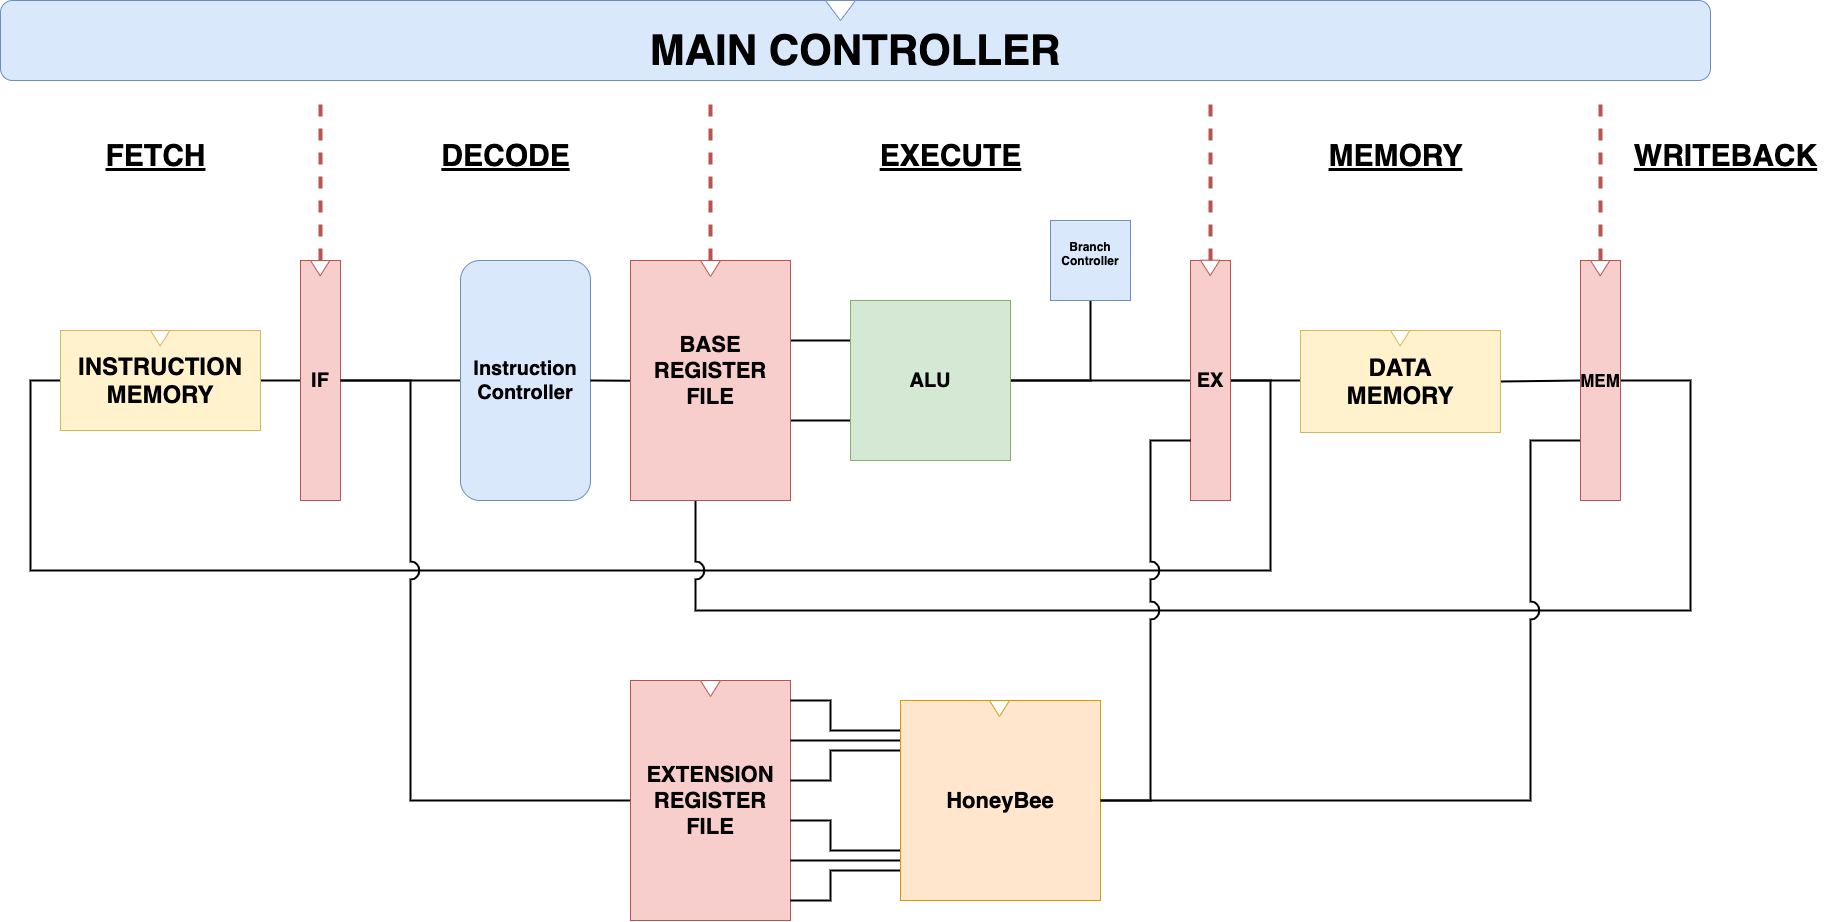
\includegraphics[width=\textwidth]{chapters/chapter4/img/philv_rv32iXedgcol.png}
\mycaption{Simplified Schematic of the RV32I\_Xedgcol PhilosophyV Core}{}
\label{fig:philv_rv32iXedgcol}
\end{center}
\end{figure}

        Implementing the Xedgcol extension was relatively simple. First, a \textbf{new register file} had to be implemented to support the new registers \texttt{e0-e5}. The register file was implemented slightly differently to normal; It was implemented with a write address port, a write data port, and then 6 data read ports that always output the value of the 6 registers. This is shown in Figure \ref{fig:refiles}.

        % @Author: AnthonyKenny98
% @Date:   2020-04-10 06:34:08
% @Last Modified by:   AnthonyKenny98
% @Last Modified time: 2020-04-10 22:44:33
\begin{figure}[H]
\begin{center}
\begin{tabular}{ccccc}


\begin{subfigure}{0.3\textwidth}
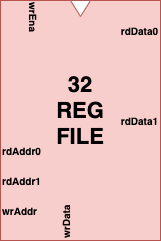
\includegraphics[width=\linewidth]{chapters/chapter4/img/regfile1.png}
\caption{}
\label{fig:regfile1_a}
\end{subfigure} & & && 

\begin{subfigure}{0.3\textwidth}
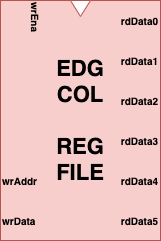
\includegraphics[width=\linewidth]{chapters/chapter4/img/regfile2.png}
\caption{}
\label{fig:regfile1_b}
\end{subfigure}\\
\end{tabular}
\mycaption{PhilosophyV Register Files}{. The 32RVI register file contains 32 registers. The ports \texttt{readData0} and \texttt{readData1} output the data held at the address provided to  \texttt{rdAddr0} and \texttt{rdAddr1} respectively. The Xedgcol register file is able to constantly output all 6 values held within it. Since the Xedgcol ISA only defines their use for one instruction, these ports can be wired directly to the HoneyBee unit.}
\label{fig:regfiles}
\end{center}
\end{figure}
        
        The \texttt{LI.e} instruction writes to this register file. In the instruction, the float immediate is only in fact the 26 most significant bits, as room must be left in the instruction for the 3 bit register address and the 3 bit opcode. As such, this float is extended with zeros in the least significant bit range before being wired to the wrData port of the register file. 
        
        Secondly, to implement the \texttt{ecol} instruction, the HoneyBee unit was added. Its 6 input ports defining the coordinates of the edge were wired directly to the output ports of the Xedgcol register file. Its 64 output bits were split to be writted to the two destination registers. The 32 \glspl{MSB} are written to rd2 in the memory stage, and the 32 \glspl{LSB} are written to rd1 in the writeback stage. Its control interface was wired to the main controller and the main controller's logic was updated. In this unoptimised processor design (to keep things simple) the processor stalls while it waits for the HoneyBee unit to complete execution.

        % @Author: AnthonyKenny98
% @Date:   2020-04-10 07:03:52
% @Last Modified by:   AnthonyKenny98
% @Last Modified time: 2020-04-10 22:48:02
\begin{figure}[H]
\begin{center}
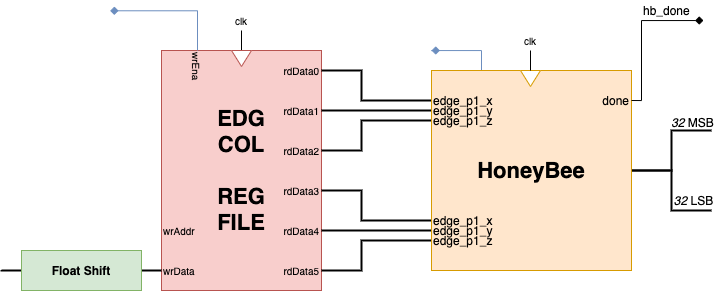
\includegraphics[width=\textwidth]{chapters/chapter4/img/honeybee_impl.png}
\mycaption{Implementation of HoneyBee in RV32I\_Xedgcol PhilosophyV}{. The data written to the register file is extended with zeros. The values of each of the 6 Xedgcol register are wired directly to the 6 input ports of HoneyBee. HoneyBee's output is written to two destination registers.}
\end{center}
\end{figure}


    \subsection{Verification}
        With the PhilosphyV core implementing the RV32I\_Xedgcol ISA, assembly tests were written to verify the viability of the Xedgcol extension. Consider an edge that is defined by the points $(0.5, 0.75, 0.25)$ and $(1.75, 1.25, 1.5)$. The assembly instructions to execute the edge collision functionality are as follows:

        \begin{verbatim}
        # Load immediate coordinate values
        LI.e px0 0.5
        LI.e py0 0.75
        LI.e pz0 0.25
        LI.e px1 1.75
        LI.e py1 1.25
        LI.e pz1 1.5
        # Execute edge collision function
        ECOL x6, x7
        \end{verbatim}

        The collision bit sequence stored in registers \texttt{x6} and \texttt{x7} can be compared against an occupancy grid map. Over multiple tests, the correct collision bits were stored in the correct registers. It was concluded from these tests that the Xedgcol extension was a viable solution.
